% main.tex
% Fichero principal de transparencias (incluye a todos los demás).

% Compilar a .pdf con LaTeX (pdflatex)
% Es necesario instalar Beamer (paquete latex-beamer en Debian)
%

% Gráficos:
% Los gráficos pueden suministrarse en PNG, JPG, TIF, PDF, MPS
% Los EPS deben convertirse a PDF (usar epstopdf)
%
\documentclass[17pt,aspectratio=169,hyperref=pdfusetitle]{beamer}
\usetheme[orchid]{Hannover}
\beamertemplatenavigationsymbolsempty
\setbeamertemplate{headline}{}
\useoutertheme{infolines}

\usepackage[spanish]{babel}
\usepackage[utf8]{inputenc}
\usepackage{graphics}
%\usepackage{amssymb} % Simbolos matematicos
%\usepackage[pdfusetitle]{hyperref}

\usepackage{chronosys}

%% two slides per page
%\usepackage{pgfpages}
%\pgfpagesuselayout{2 on 1}[a4paper,border shrink=5mm]

\newcommand\YUGE{\fontsize{48}{60}\selectfont}

\newcommand{\secimage}{figs/bookpages}
\AtBeginSection[]
{
  {
    \usebackgroundtemplate{\includegraphics[width=\paperwidth,height=\paperheight]{\secimage}}
    \begin{frame}<beamer>

      \begin{center}
        {\YUGE\bf\insertsection}
      \end{center}
    \end{frame}
  }
  \renewcommand{\secimage}{figs/bookpages}
}


\title[Un rato con amigos]{Un rato con unos amigos}
\subtitle{Lección magistral, lo llaman...}
\author[Jesús M. González Barahona]{Jesús M. González Barahona \\
@jgbarah}
\institute[URJC]{Universidad Rey Juan Carlos \\
  \url{http://github.com/jgbarah/presentations}}

\date{6 de abril de 2018}

\begin{document}

%\begin{frame}[label=firstframe]
\begin{frame}
  \maketitle
\end{frame}


\begin{frame}

  {\em
    Ante todo, gracias a los culpables:

    \begin{flushright}
    Gregorio Robles \\
    Pedro de las Heras \\
    Israel Herraiz \\
    Daniel Izquierdo \\
    Felipe Ortega \\
    Antonio Reinoso \\
    \end{flushright}
  }
\end{frame}

\begin{frame}

  {\em
    \begin{center}
      %\begin{quote}
      ``Jesús nos contará a qué ha dedicado \\
      los últimos 20 años \\
      y qué piensa hacer en \\
      los (al menos) siguientes 20''\\
      %\end{quote}
    \end{center}
  }
\end{frame}

\begin{frame}

  {\em \Huge
    \begin{center}
      Uffff
    \end{center}
  }
\end{frame}


\frame{
\tableofcontents
}


%%%%%%%%%%%%%%%%%%%%%%%%%%%%%%%%%%%%%%%%%%%%%%%%%%%%%%%%%%%%%%%%
%%%%%%%%%%%%%%%%%%%%%%%%%%%%%%%%%%%%%%%%%%%%%%%%%%%%%%%%%%%%%%%%
% lista de temas                                               %
%%%%%%%%%%%%%%%%%%%%%%%%%%%%%%%%%%%%%%%%%%%%%%%%%%%%%%%%%%%%%%%%
%%%%%%%%%%%%%%%%%%%%%%%%%%%%%%%%%%%%%%%%%%%%%%%%%%%%%%%%%%%%%%%%
%% Pasado
%%

\definecolor{lightviolet}{HTML}{F4AFF4}
\definecolor{lightorange}{HTML}{FFA17F}
\definecolor{lightgreen}{HTML}{98FB98}
\definecolor{lightred}{HTML}{FF5C5C}
\definecolor{lightblue}{HTML}{89AFCF}
\definecolor{lightbrown}{HTML}{B58868}

%%-----------------------------------------
%%-----------------------------------------
\section{Pasado}

\begin{flushright}
{\em
  ¿Quiénes somos? \\
  ¿De dónde venimos? \\
  ¿Adónde vamos? \\
}
~ \\
Siniestro Total \\
\end{flushright}


%%-----------------------------------------
\begin{frame}[fragile]
  \frametitle{La suerte de estar en el sitio adecuado}

  \begin{center}
  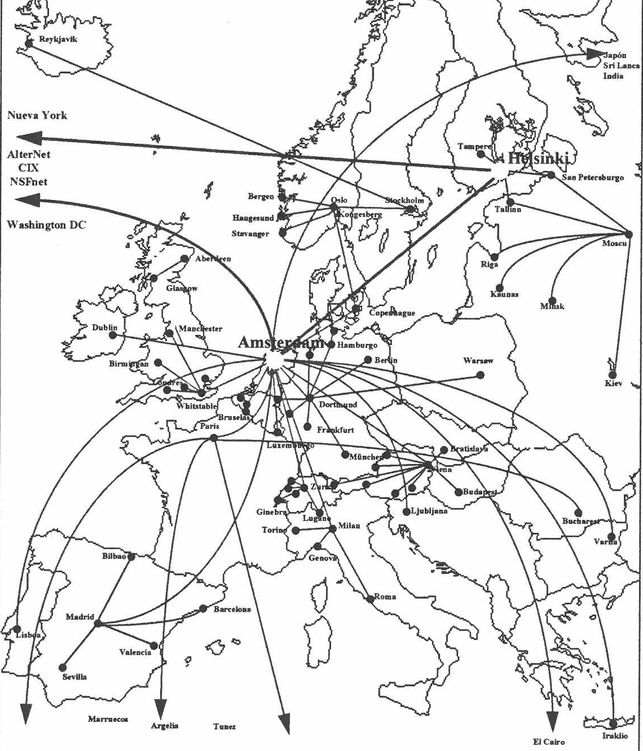
\includegraphics[height=6cm]{figs/eunet}
  \end{center}  
  
\end{frame}

%%-----------------------------------------
\begin{frame}[fragile]
  \frametitle{La suerte de estar en el momento adecuado}

  \begin{center}
  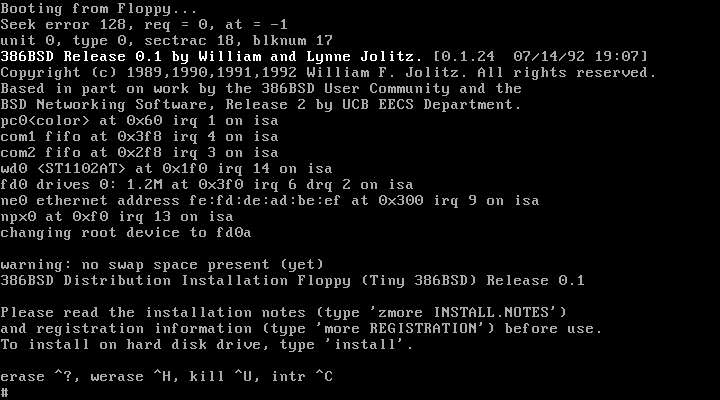
\includegraphics[height=6cm]{figs/386BSD-installer}
  \end{center}  
  
\end{frame}

%%-----------------------------------------
\begin{frame}[fragile]
  \frametitle{La suerte de tener buenos maestros}

  \begin{center}
  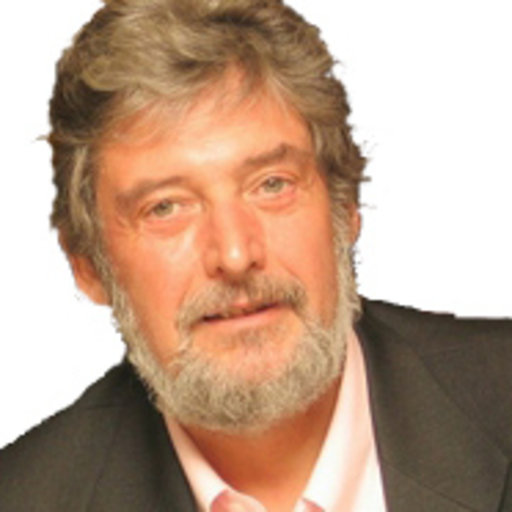
\includegraphics[height=3.5cm]{figs/foto-aalvarez}
  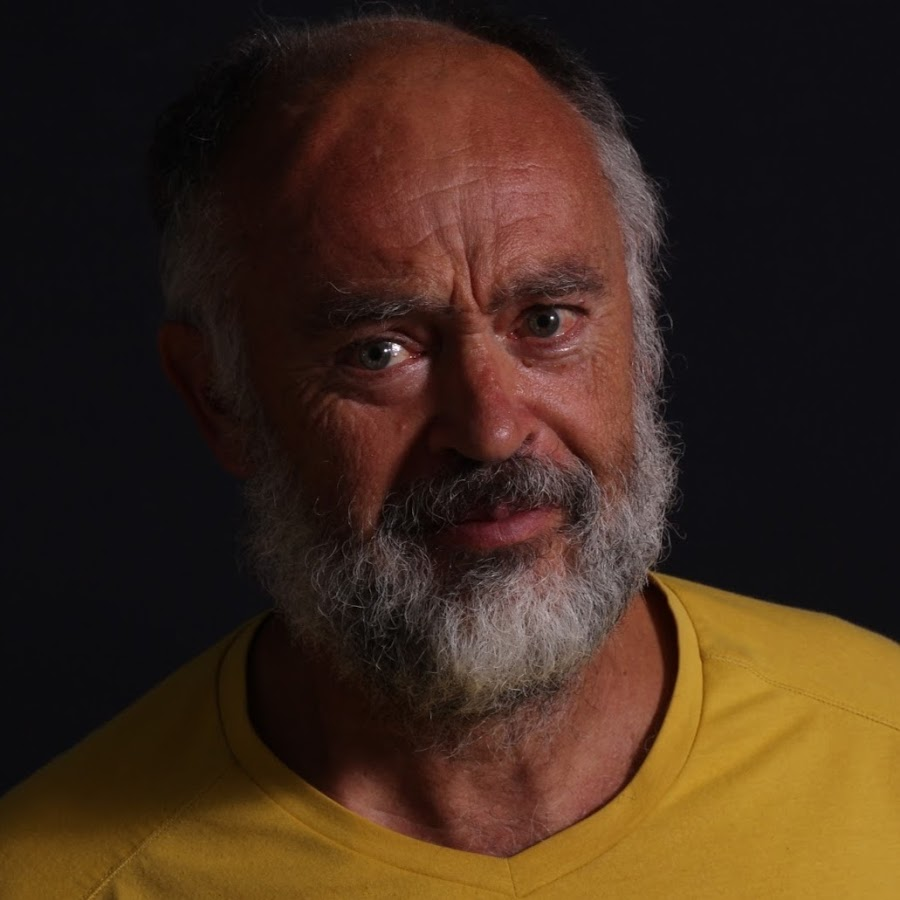
\includegraphics[height=3.5cm]{figs/foto-jseoane}
  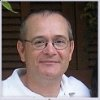
\includegraphics[height=3.5cm]{figs/foto-sarevalo}
  \end{center}  
  
\end{frame}

%%-----------------------------------------
\begin{frame}[fragile]
  \frametitle{La suerte de que te hayan preparado el camino}

  \begin{center}
  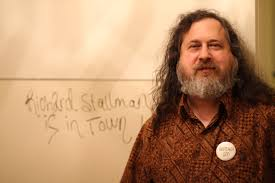
\includegraphics[height=6cm]{figs/foto-rms}
  \end{center}  
  
\end{frame}

%%-----------------------------------------
\begin{frame}[fragile]
  \frametitle{Mi vida (académica)}

  % Definition of the chronology element
%  \startchronology[align=left, startyear=1986,stopyear=2017, height=0pt, startdate=false, stopdate=false, dateselevation=0pt, arrow=false, box=true]
  %
  %  \chronograduation[event][dateselevation=0pt]{1}
  \startchronology[startyear=1984,stopyear=2017,dates=false,color=white]
  % Periods and events

  \chronoperiode[textstyle=\raggedleft\colorbox{gray!30}, color=gray, startdate=false, bottomdepth=0pt, topheight=8pt, textdepth=-25pt,dateselevation=16pt, stopdate=false]{1986}{1992}{Ing. Telecom (UPM)}

  \chronoevent[colorbox=gray!30,conversionmonth=false, datesseparation=/, markdepth=3cm]{12/1991}{Ing. Telecomunicación (UPM)}

  \chronoperiode[textstyle=\raggedleft\colorbox{gray!30}, color=gray, startdate=false, bottomdepth=0pt, topheight=8pt, textdepth=-45pt,dateselevation=16pt, stopdate=false]{1993}{1999}{Doctorado (UPM)}

  \chronoevent[colorbox=gray!30,conversionmonth=false,datesseparation=/, markdepth=1.5cm]{12/1998}{Doctor Ing. Telecomunicación}

  \chronoperiode[textstyle=\colorbox{lightviolet}, color=lightviolet, startdate=false, bottomdepth=10pt, topheight=18pt, textdepth=-55pt, dateselevation=12pt,stopdate=false]{1992}{2000}{UC3M}

  \chronoperiode[textstyle=\colorbox{lightviolet}, color=lightviolet, startdate=false, bottomdepth=10pt, topheight=18pt, textdepth=-55pt, dateselevation=12pt,stopdate=false]{2000}{2017}{URJC}

  \chronoevent[colorbox=gray!30,conversionmonth=false,datesseparation=/, markdepth=.1cm]{05/2001}{Plaza TU}

  \chronoevent[colorbox=gray!30,conversionmonth=false,datesseparation=/, markdepth=.1cm]{05/2015}{Habilitación CU}

  \stopchronology

\end{frame}


%%-----------------------------------------
\begin{frame}[fragile]
  \frametitle{Una vida docente}

  {\small
  ~~~~~~~UCAR~~~~~~~~~~~~~~~~~~~~~~~~~~~~~~~URJC
  }
  
  \vspace{.2cm}
  
  {\footnotesize
  \startchronology[startyear=1992,stopyear=2018,dates=true, color=white, width=.9\textwidth]

  % UC3M Informatica
  \chronoperiode[color=lightred, startdate=false, stopdate=false, bottomdepth=0pt, topheight=8pt]{1992}{1999}{}

  \chronoevent[barre=false, colorbox=lightred, markdepth=1.2cm, date=false, textwidth=2.4cm]{1/1995}{Informática}

  % UC3M Industriales
  \chronoperiode[color=lightred, startdate=false, stopdate=false, bottomdepth=10pt, topheight=18pt]{1997}{1999}{}

  \chronoevent[barre=false, colorbox=lightred, markdepth=.7cm, date=false, textwidth=1.9cm]{1/1998}{Industriales}

  % UC3M Doctorado
  \chronoperiode[color=lightgreen, startdate=false, stopdate=false, bottomdepth=20pt, topheight=28pt]{1997}{1999}{}

  \chronoevent[barre=false, colorbox=lightgreen, markdepth=.2cm, date=false, textwidth=1.9cm]{1/1998}{Doctorado}

  % URJC Grado Ciencias Salud
  \chronoperiode[color=lightred, startdate=false, stopdate=false, bottomdepth=60pt, topheight=68pt]{1999}{2005}{}

  \chronoevent[barre=false, colorbox=lightred, markdepth=1.6cm, date=false, textwidth=2cm]{7/2001}{C. Salud}

  % URJC Grado Informática
  \chronoperiode[color=lightred, startdate=false, stopdate=false, bottomdepth=70pt, topheight=78pt]{1999}{2011}{}

  \chronoevent[barre=false, colorbox=lightred, markdepth=1.2cm, date=false, textwidth=2.5cm]{1/2005}{Informática}

  % URJC Grado Teleco
  \chronoperiode[color=lightred, startdate=false, stopdate=false, bottomdepth=80pt, topheight=88pt]{2003}{2018}{}

  \chronoevent[barre=false, colorbox=lightred, markdepth=1.6cm, date=false, textwidth=2cm]{1/2010}{Teleco}

  % URJC Doctorado Informatica
  \chronoperiode[color=lightgreen, startdate=false, stopdate=false, bottomdepth=30pt, topheight=38pt]{2001}{2006}{}

  \chronoevent[barre=false, colorbox=lightgreen, markdepth=.2cm, date=false, textwidth=1.9cm]{7/2003}{Doctorado}

  % URJC Máster RSCM URJC
  \chronoperiode[color=lightviolet, startdate=false, stopdate=false, bottomdepth=40pt, topheight=48pt]{2006}{2011}{}

  \chronoevent[barre=false, colorbox=lightviolet, markdepth=.7cm, date=false, textwidth=2.5cm]{7/2008}{Máster RSCM}

  % URJC Máster Software Libre URJC
  \chronoperiode[color=lightviolet, startdate=false, stopdate=false, bottomdepth=50pt, topheight=58pt]{2006}{2014}{}

  \chronoevent[barre=false, colorbox=lightviolet, markdepth=.2cm, date=false, textwidth=1.9cm]{1/2009}{Máster SL}

  \stopchronology
  }
\end{frame}



%%-----------------------------------------
\begin{frame}[fragile]
  \frametitle{UC3M (1992-1999)}

  \begin{center}
  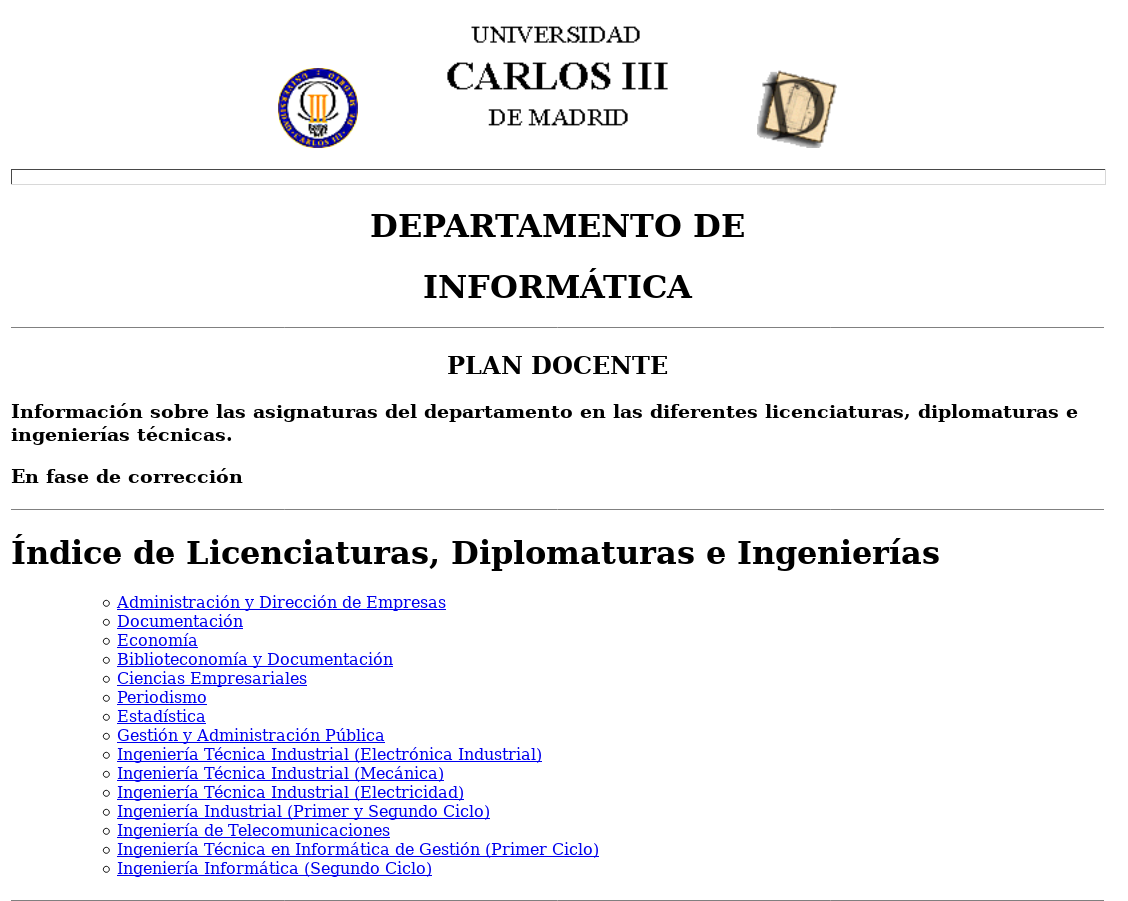
\includegraphics[height=8cm]{figs/inf-uc3m}
  \end{center}  
  
\end{frame}

%%-----------------------------------------
\begin{frame}[fragile]
  \frametitle{Laboratorios con software libre (1993-2005)}

  \begin{center}
  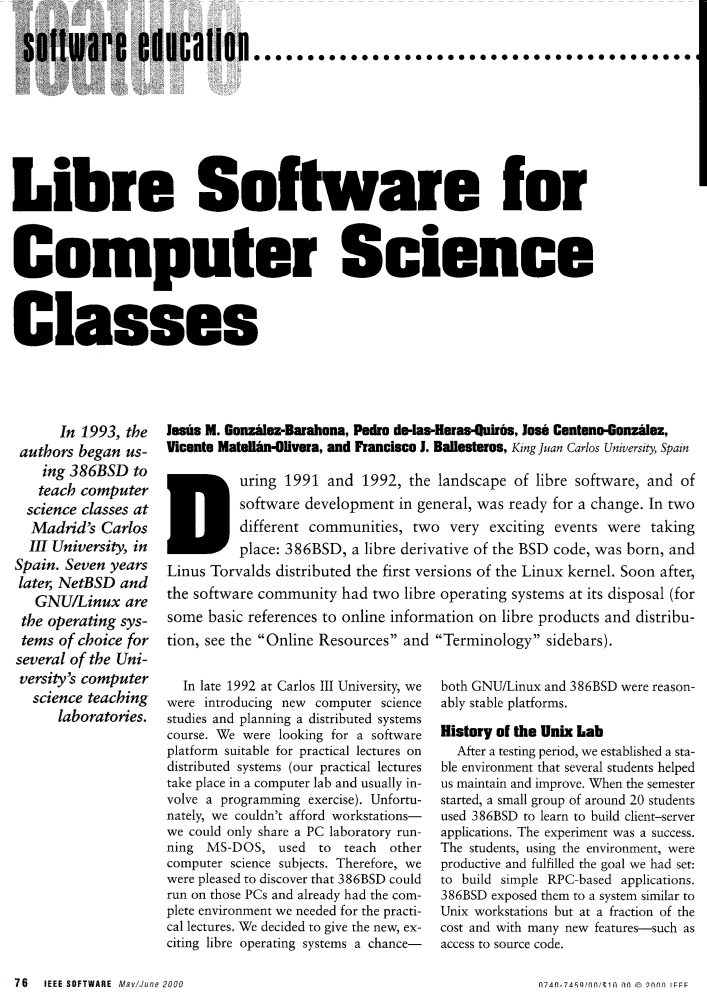
\includegraphics[height=8cm]{figs/libre-classes}
  \end{center}  
  
\end{frame}

%%-----------------------------------------
\begin{frame}[fragile]
  \frametitle{GSyC (1995-)}

  \begin{center}
  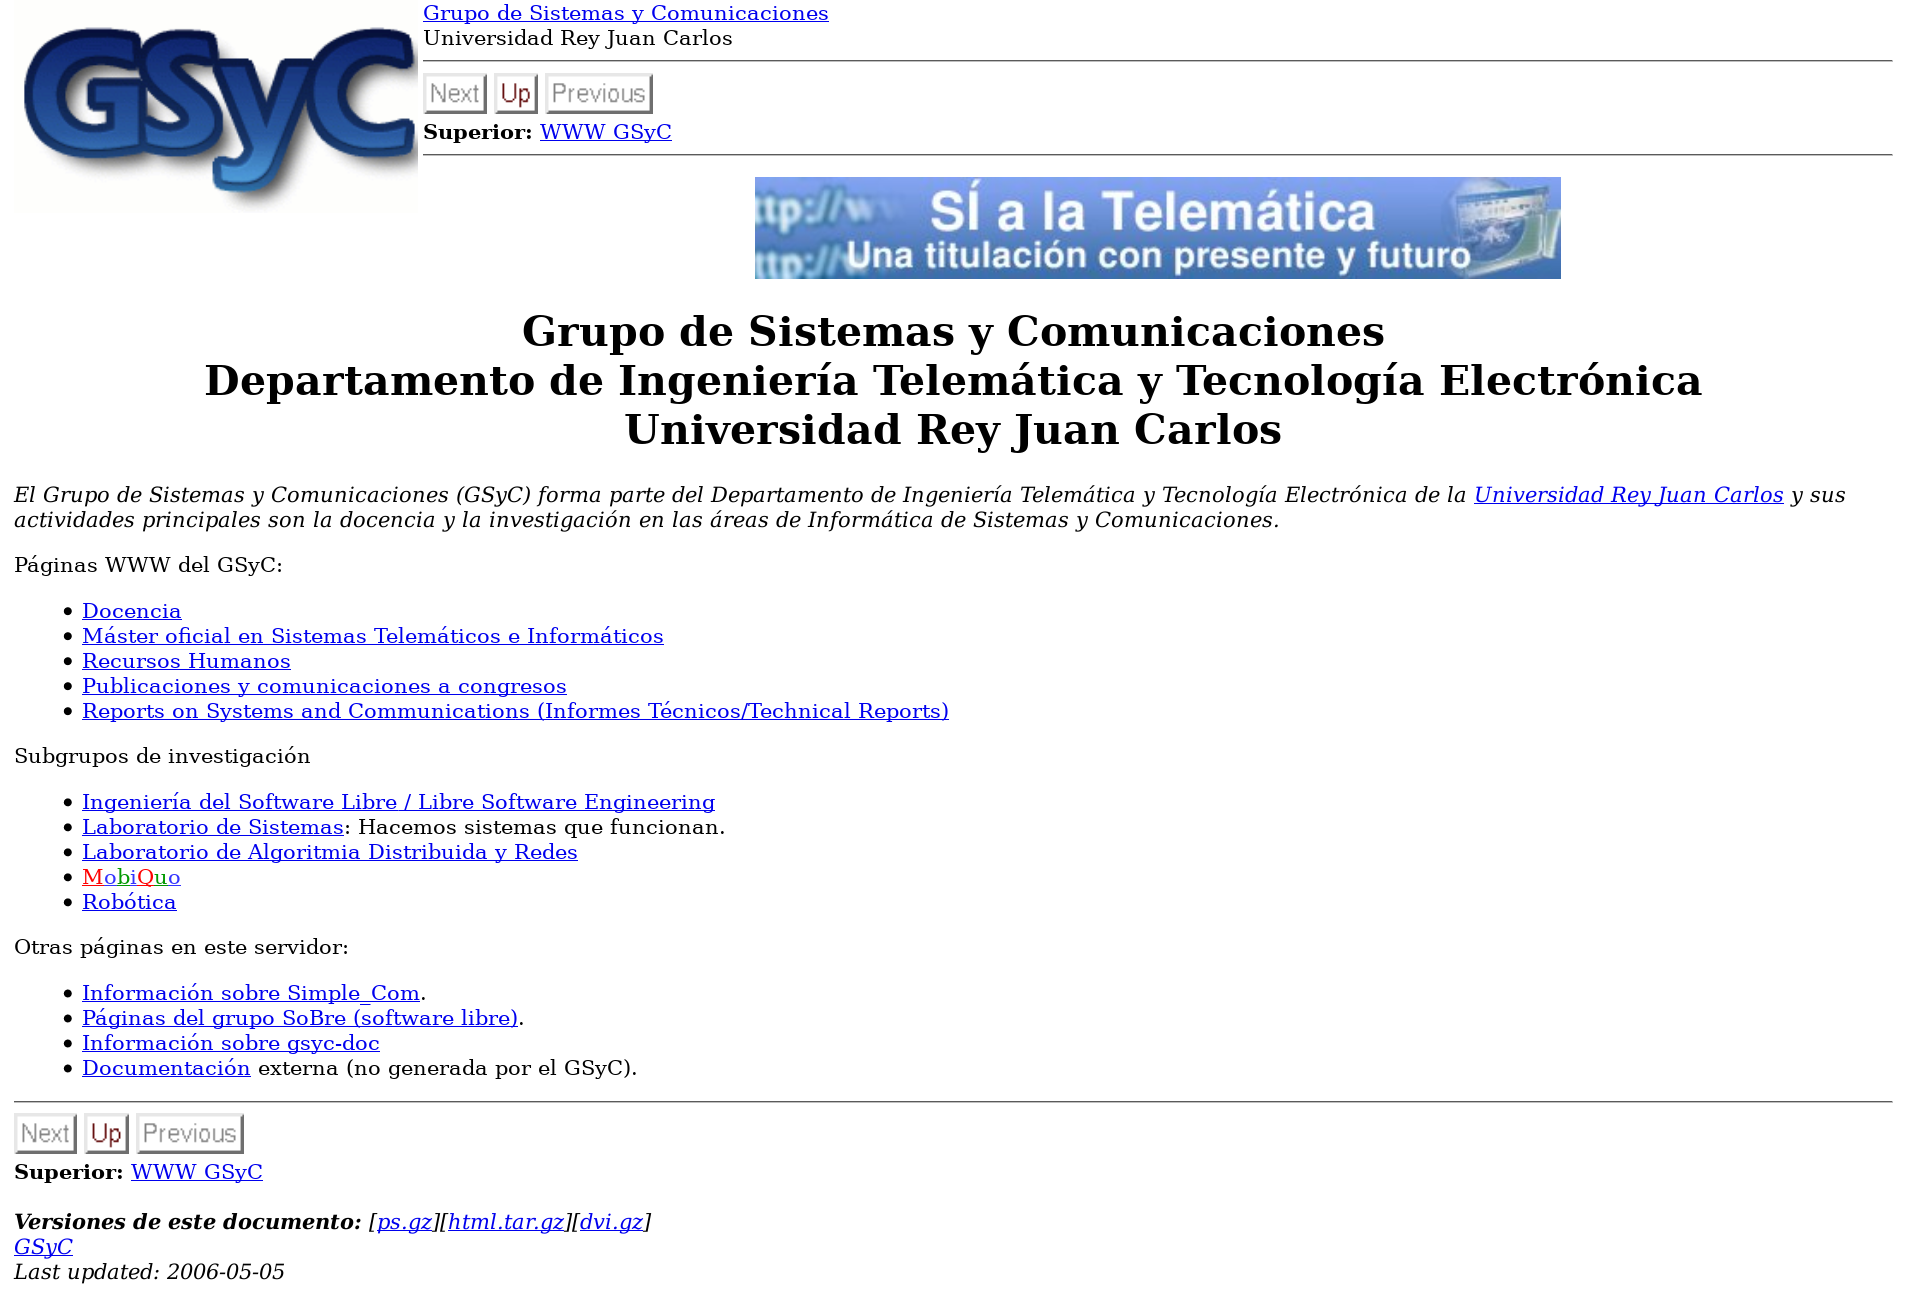
\includegraphics[height=8cm]{figs/gsyc}
  \end{center}  
  
\end{frame}

%%-----------------------------------------
\begin{frame}[fragile]
  \frametitle{Tesis y Lower\_Layer (1995-2002)}

  \begin{center}
  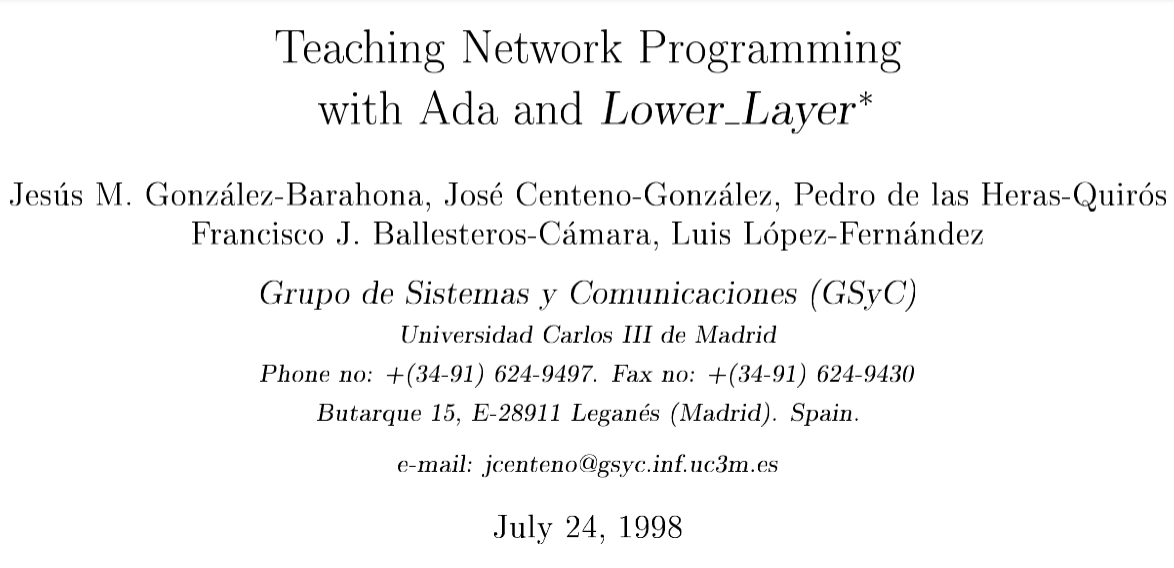
\includegraphics[width=12cm]{figs/lower-layer}
  \end{center}  
  
\end{frame}

%%-----------------------------------------
\begin{frame}[fragile]
  \frametitle{Software libre en Europa (1997-2005)}

  \begin{center}
  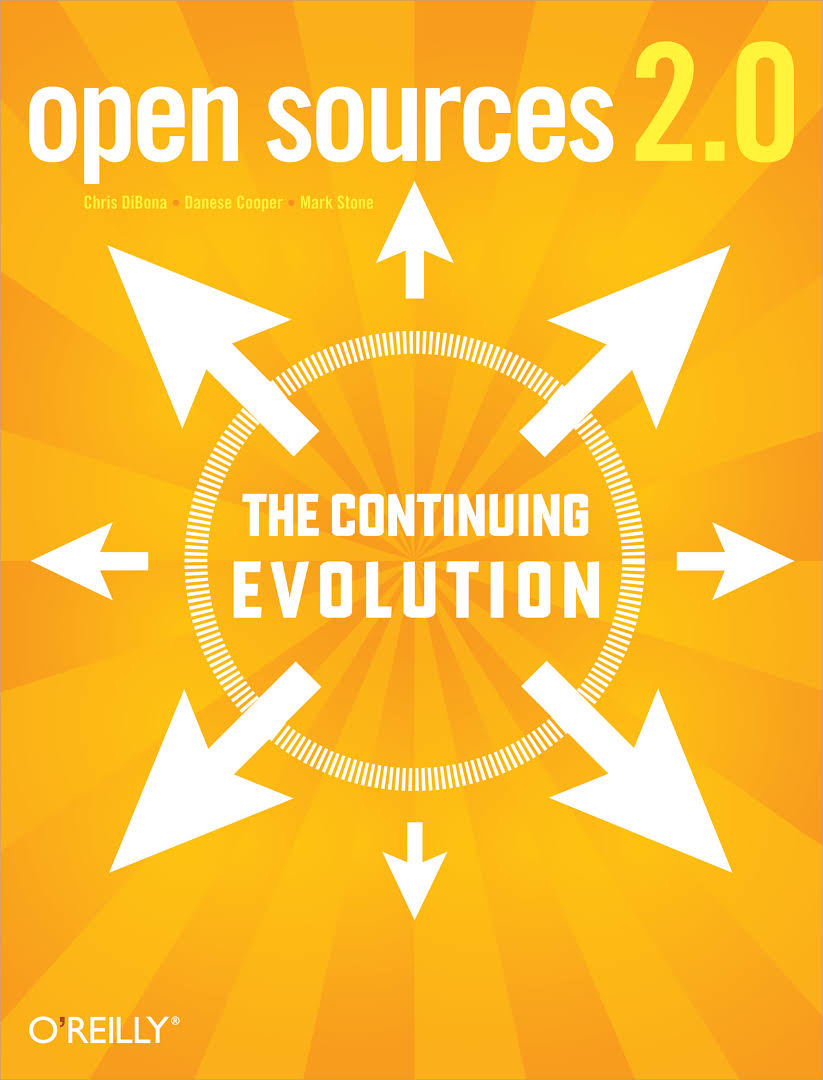
\includegraphics[height=8cm]{figs/opensources}
  \end{center}  
  
\end{frame}

%%-----------------------------------------
\begin{frame}[fragile]
  \frametitle{ESCET (URJC) (1999-2011)}

  \begin{center}
  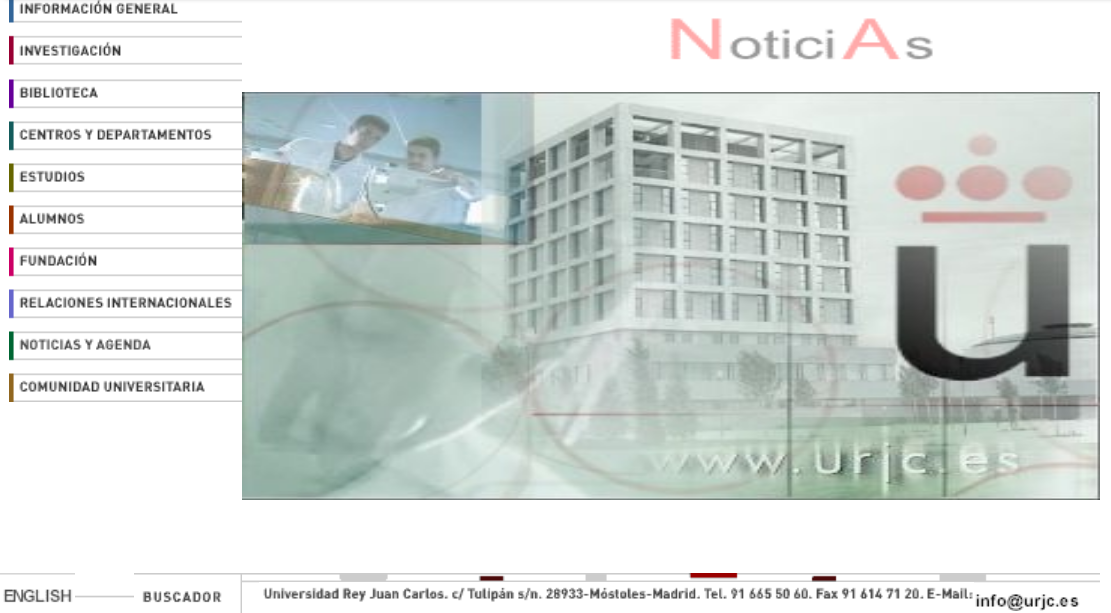
\includegraphics[width=11cm]{figs/web-urjc-2001}
  \end{center}  
  
\end{frame}

%%-----------------------------------------
\begin{frame}[fragile]
  \frametitle{Countando patatas (2000-2001)}

  \begin{center}
  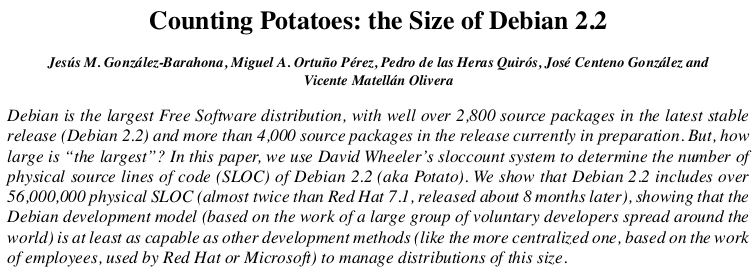
\includegraphics[width=12cm]{figs/counting-potatos}

  
\includegraphics[width=6cm]{figs/upgrade}
  \end{center}  
  
\end{frame}

%%-----------------------------------------
\begin{frame}[fragile]
  \frametitle{Uso de datos de CVS (2001-2003)}

  \begin{center}
  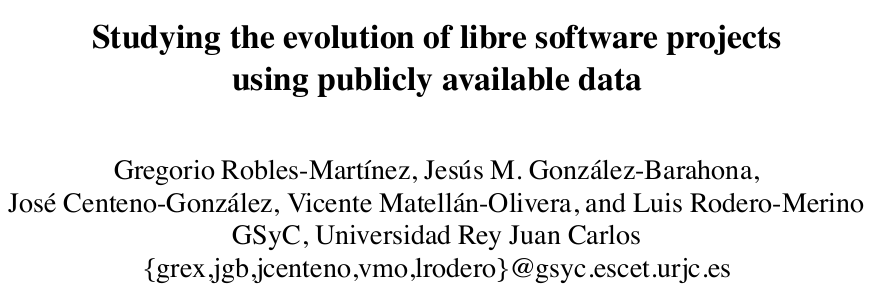
\includegraphics[width=12cm]{figs/evolution-data}
  \end{center}  
  
\end{frame}

%%-----------------------------------------
\begin{frame}[fragile]
  \frametitle{GSyC/LibreSoft (2002-)}

  \begin{center}
  
\includegraphics[height=8cm]{figs/libresoft}
  \end{center}  
  
\end{frame}

%%-----------------------------------------
\begin{frame}[fragile]
  \frametitle{CVSAnalY (2002-2015)}

  \begin{center}
  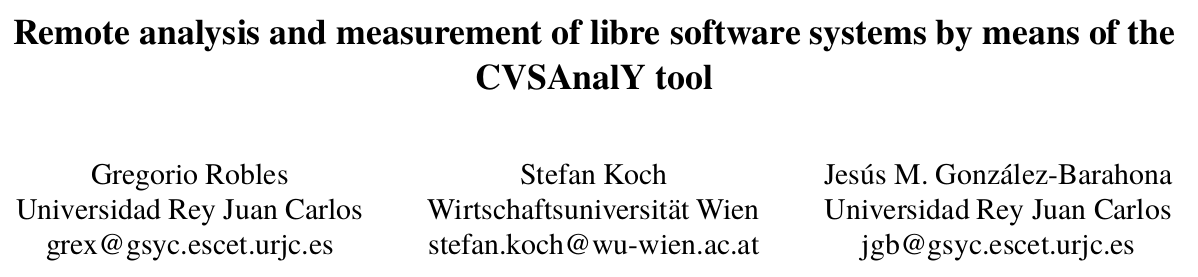
\includegraphics[width=12cm]{figs/cvsanaly}
  \end{center}  
  
\end{frame}

%%-----------------------------------------
\begin{frame}[fragile]
  \frametitle{ETSIT (URJC) (2003-)}

  \begin{center}
  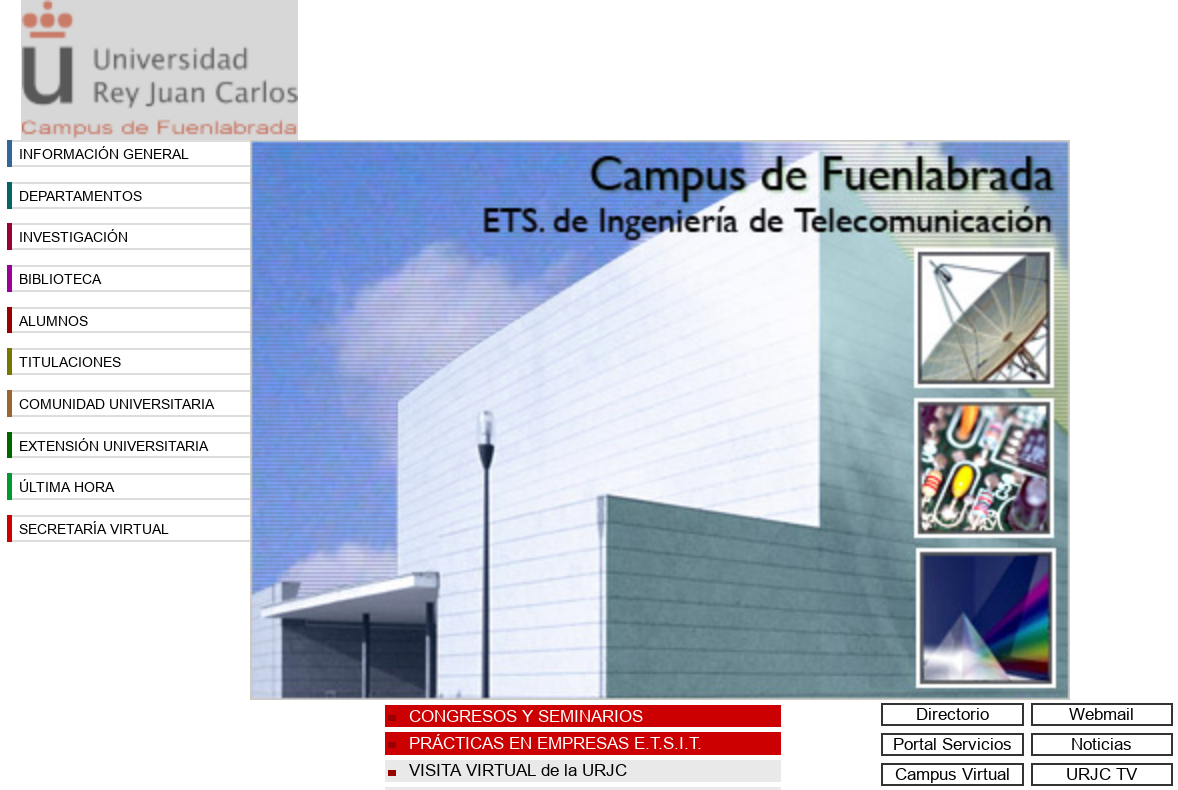
\includegraphics[width=12cm]{figs/etsit-urjc}
  \end{center}  
  
\end{frame}


%%-----------------------------------------
\begin{frame}[fragile]
  \frametitle{Macro-evolución (2005-2008)}

  \begin{center}
  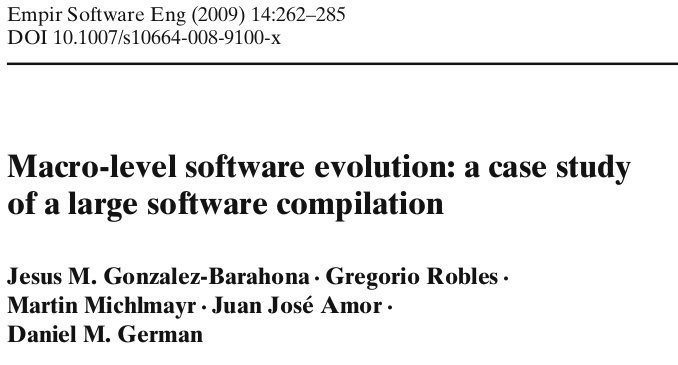
\includegraphics[width=12cm]{figs/macro-evolution}
  \end{center}  
  
\end{frame}

%%-----------------------------------------
\begin{frame}[fragile]
  \frametitle{Docencia sobre software libre (2002-2008)}

  \begin{center}
  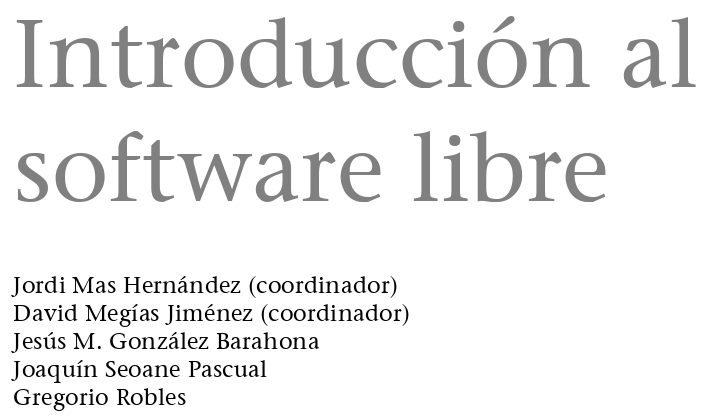
\includegraphics[width=12cm]{figs/intro-sobre}
  \end{center}  
  
\end{frame}

%%-----------------------------------------
\begin{frame}[fragile]
  \frametitle{FLOSSMetrics (2006-2009)}

  \begin{center}
  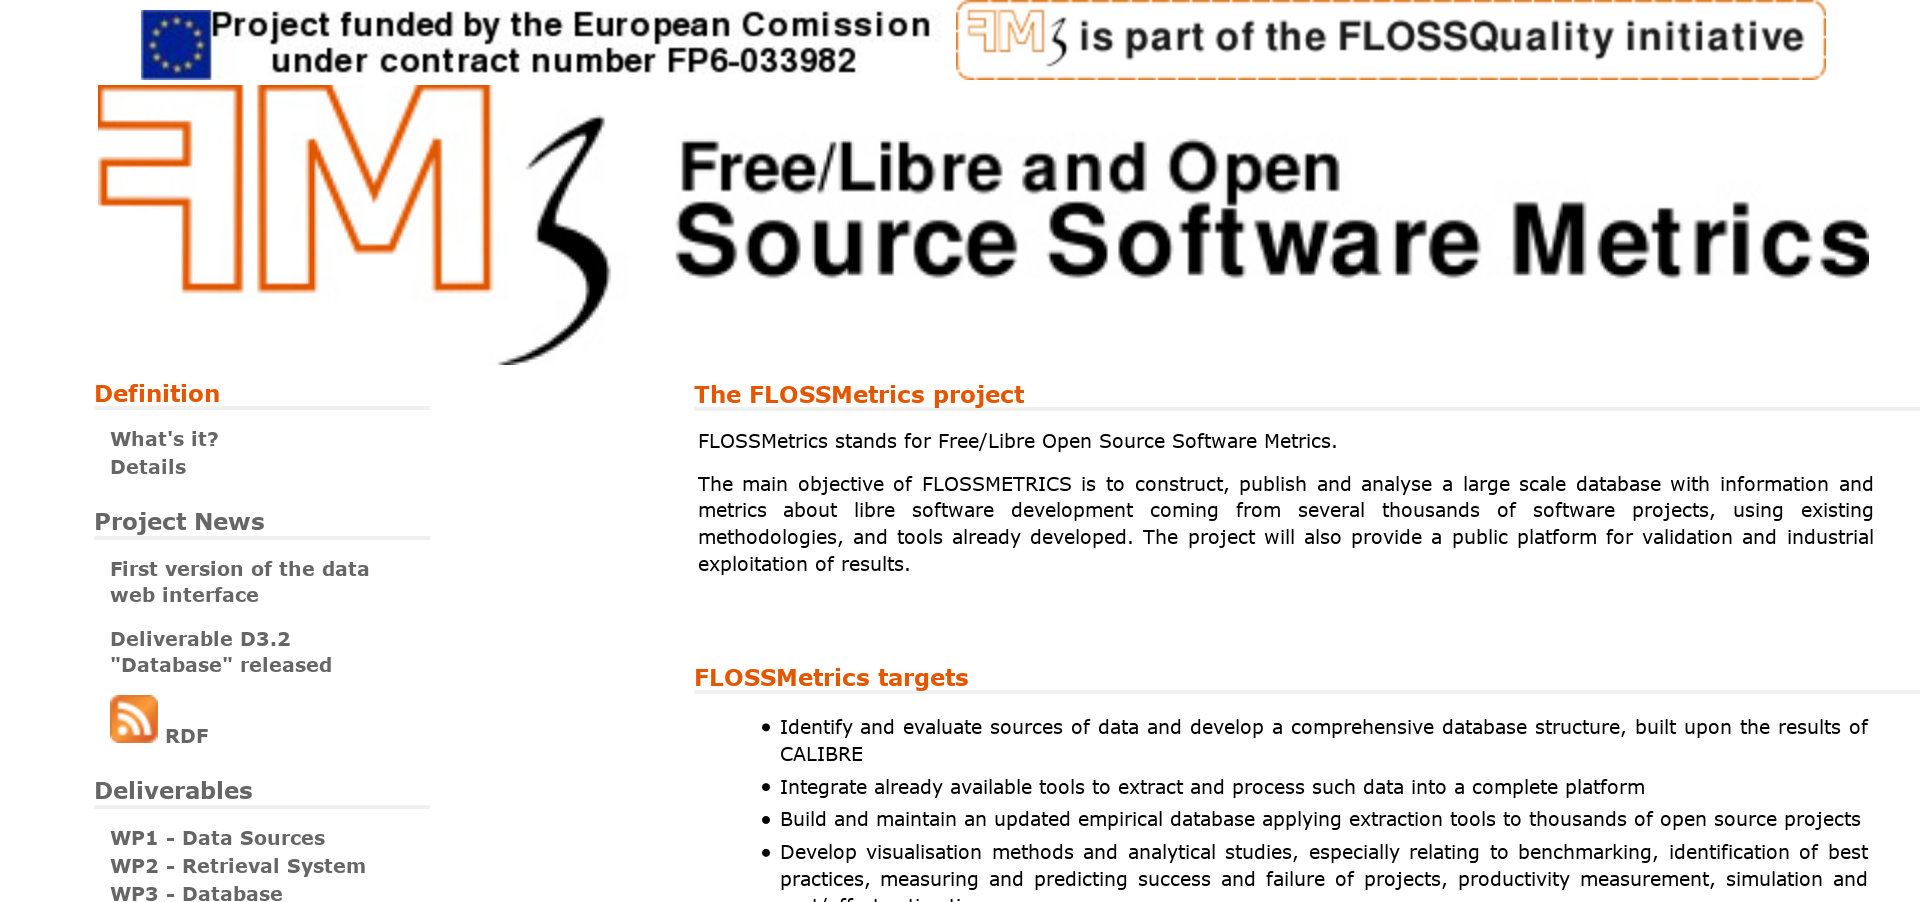
\includegraphics[width=12cm]{figs/flossmetrics}
  \end{center}  
  
\end{frame}

%%-----------------------------------------
\begin{frame}[fragile]
  \frametitle{Estudios sobre Wikipedia (2007-2009)}

  \begin{center}
  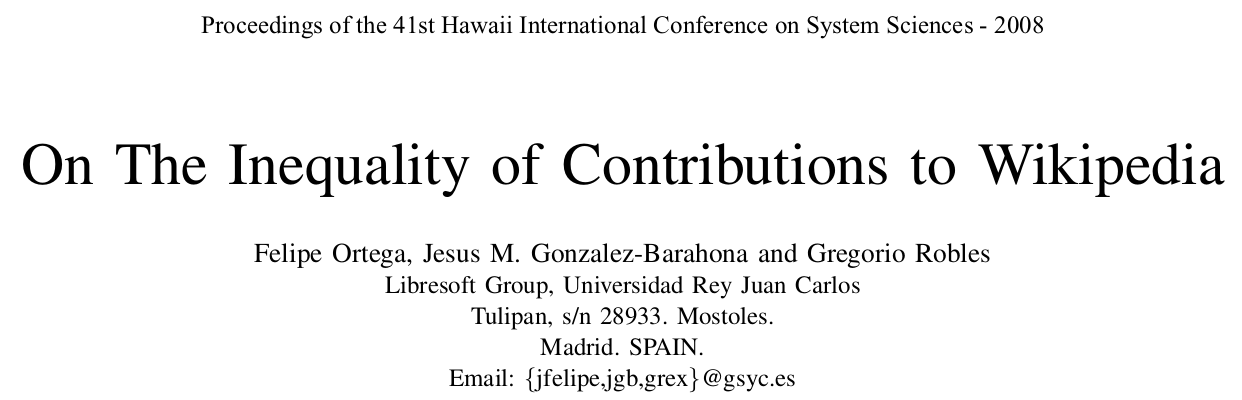
\includegraphics[width=12cm]{figs/wikipedia}
  \end{center}  
  
\end{frame}

%%-----------------------------------------
\begin{frame}[fragile]
  \frametitle{Reproducibilidad (2008-2012)}

  \begin{center}
  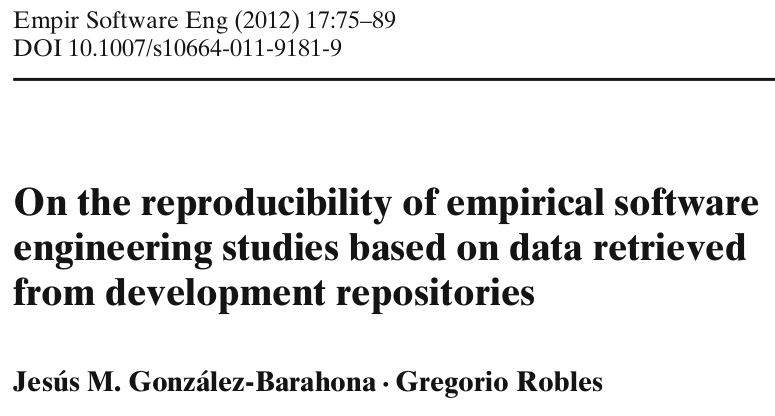
\includegraphics[width=12cm]{figs/reproducibility}
  \end{center}  
  
\end{frame}

%%-----------------------------------------
\begin{frame}[fragile]
  \frametitle{Evolución basada en datos (2008-2013)}

  \begin{center}
  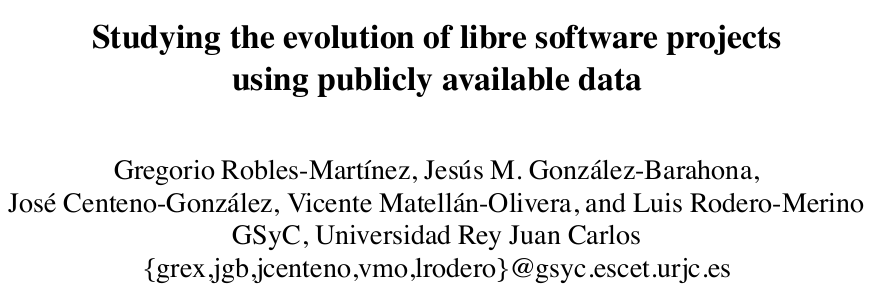
\includegraphics[width=12cm]{figs/evolution-data}
  \end{center}  
  
\end{frame}

%%-----------------------------------------
\begin{frame}[fragile]
  \frametitle{Empresas y comunidades (2010-2013)}

  \begin{center}
  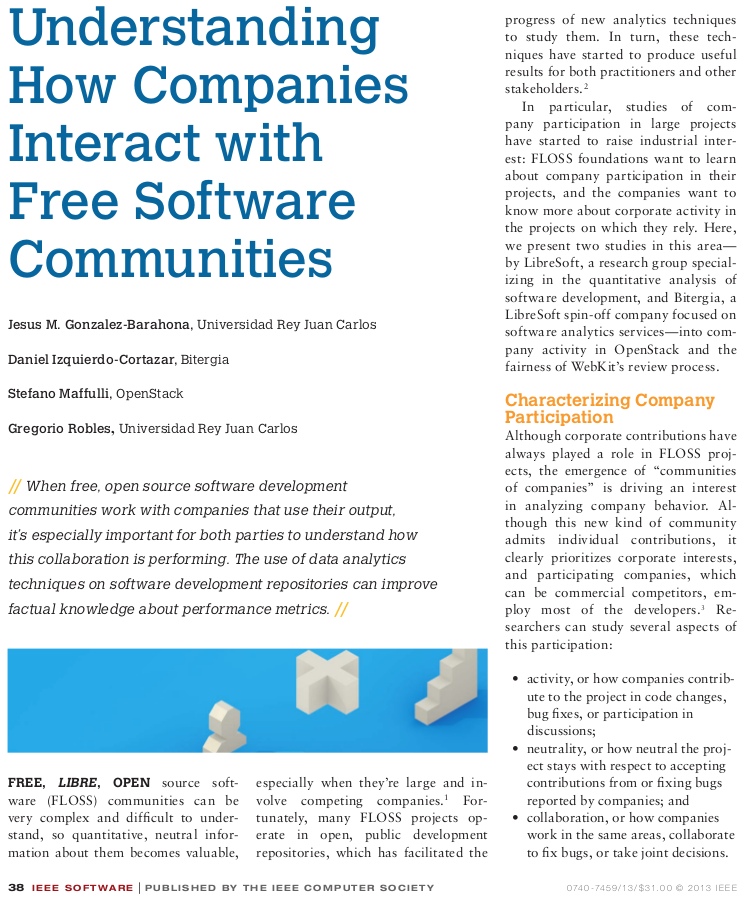
\includegraphics[width=12cm]{figs/software-companies}
  \end{center}  
  
\end{frame}

%%-----------------------------------------
\begin{frame}[fragile]
  \frametitle{MetricsGrimoire (2002-2015)}

  \begin{center}
  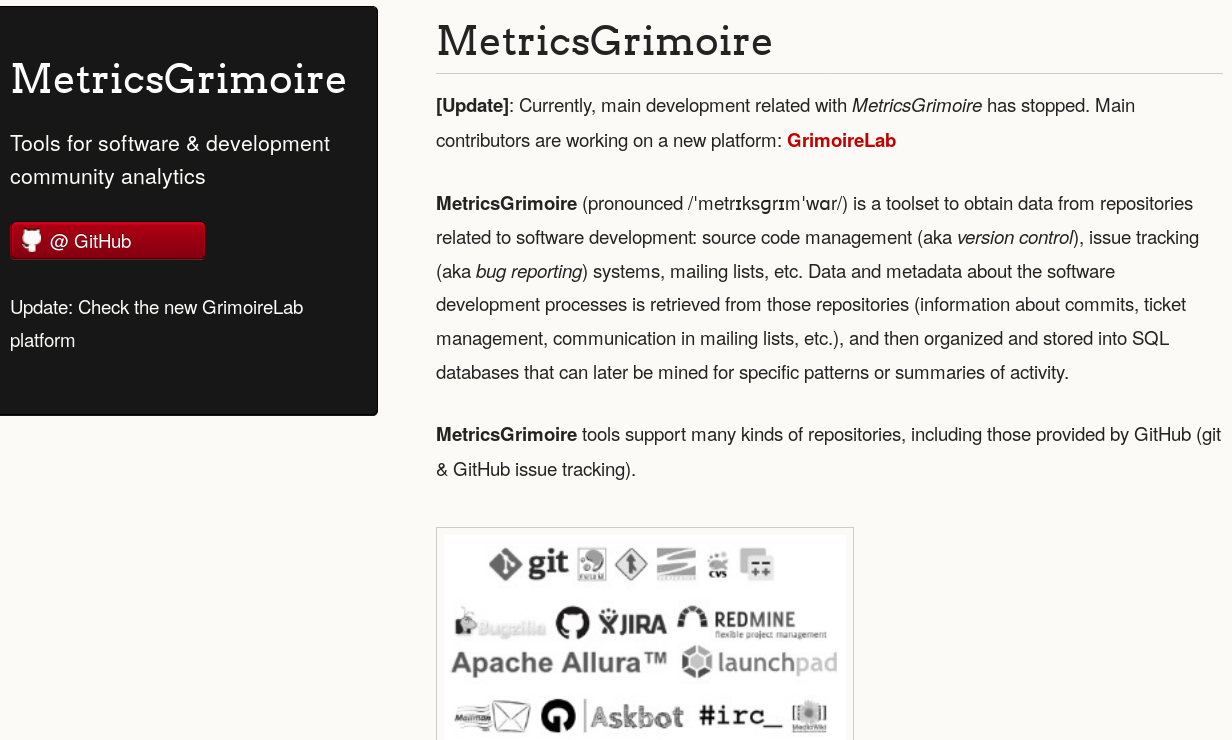
\includegraphics[width=12cm]{figs/metricsgrimoire}
  \end{center}  
  
\end{frame}

%%-----------------------------------------
\begin{frame}[fragile]
  \frametitle{Bitergia (2012-)}

  \begin{center}
  
\includegraphics[width=12cm]{figs/bitergia}
  \end{center}  
  
\end{frame}

%%-----------------------------------------
\begin{frame}[fragile]
  \frametitle{GrimoireLab (2014-)}

  \begin{center}
  
\includegraphics[width=12cm]{figs/grimoirelab}
  \end{center}  
  
\end{frame}

%%-----------------------------------------
\begin{frame}[fragile]

  \begin{center}
  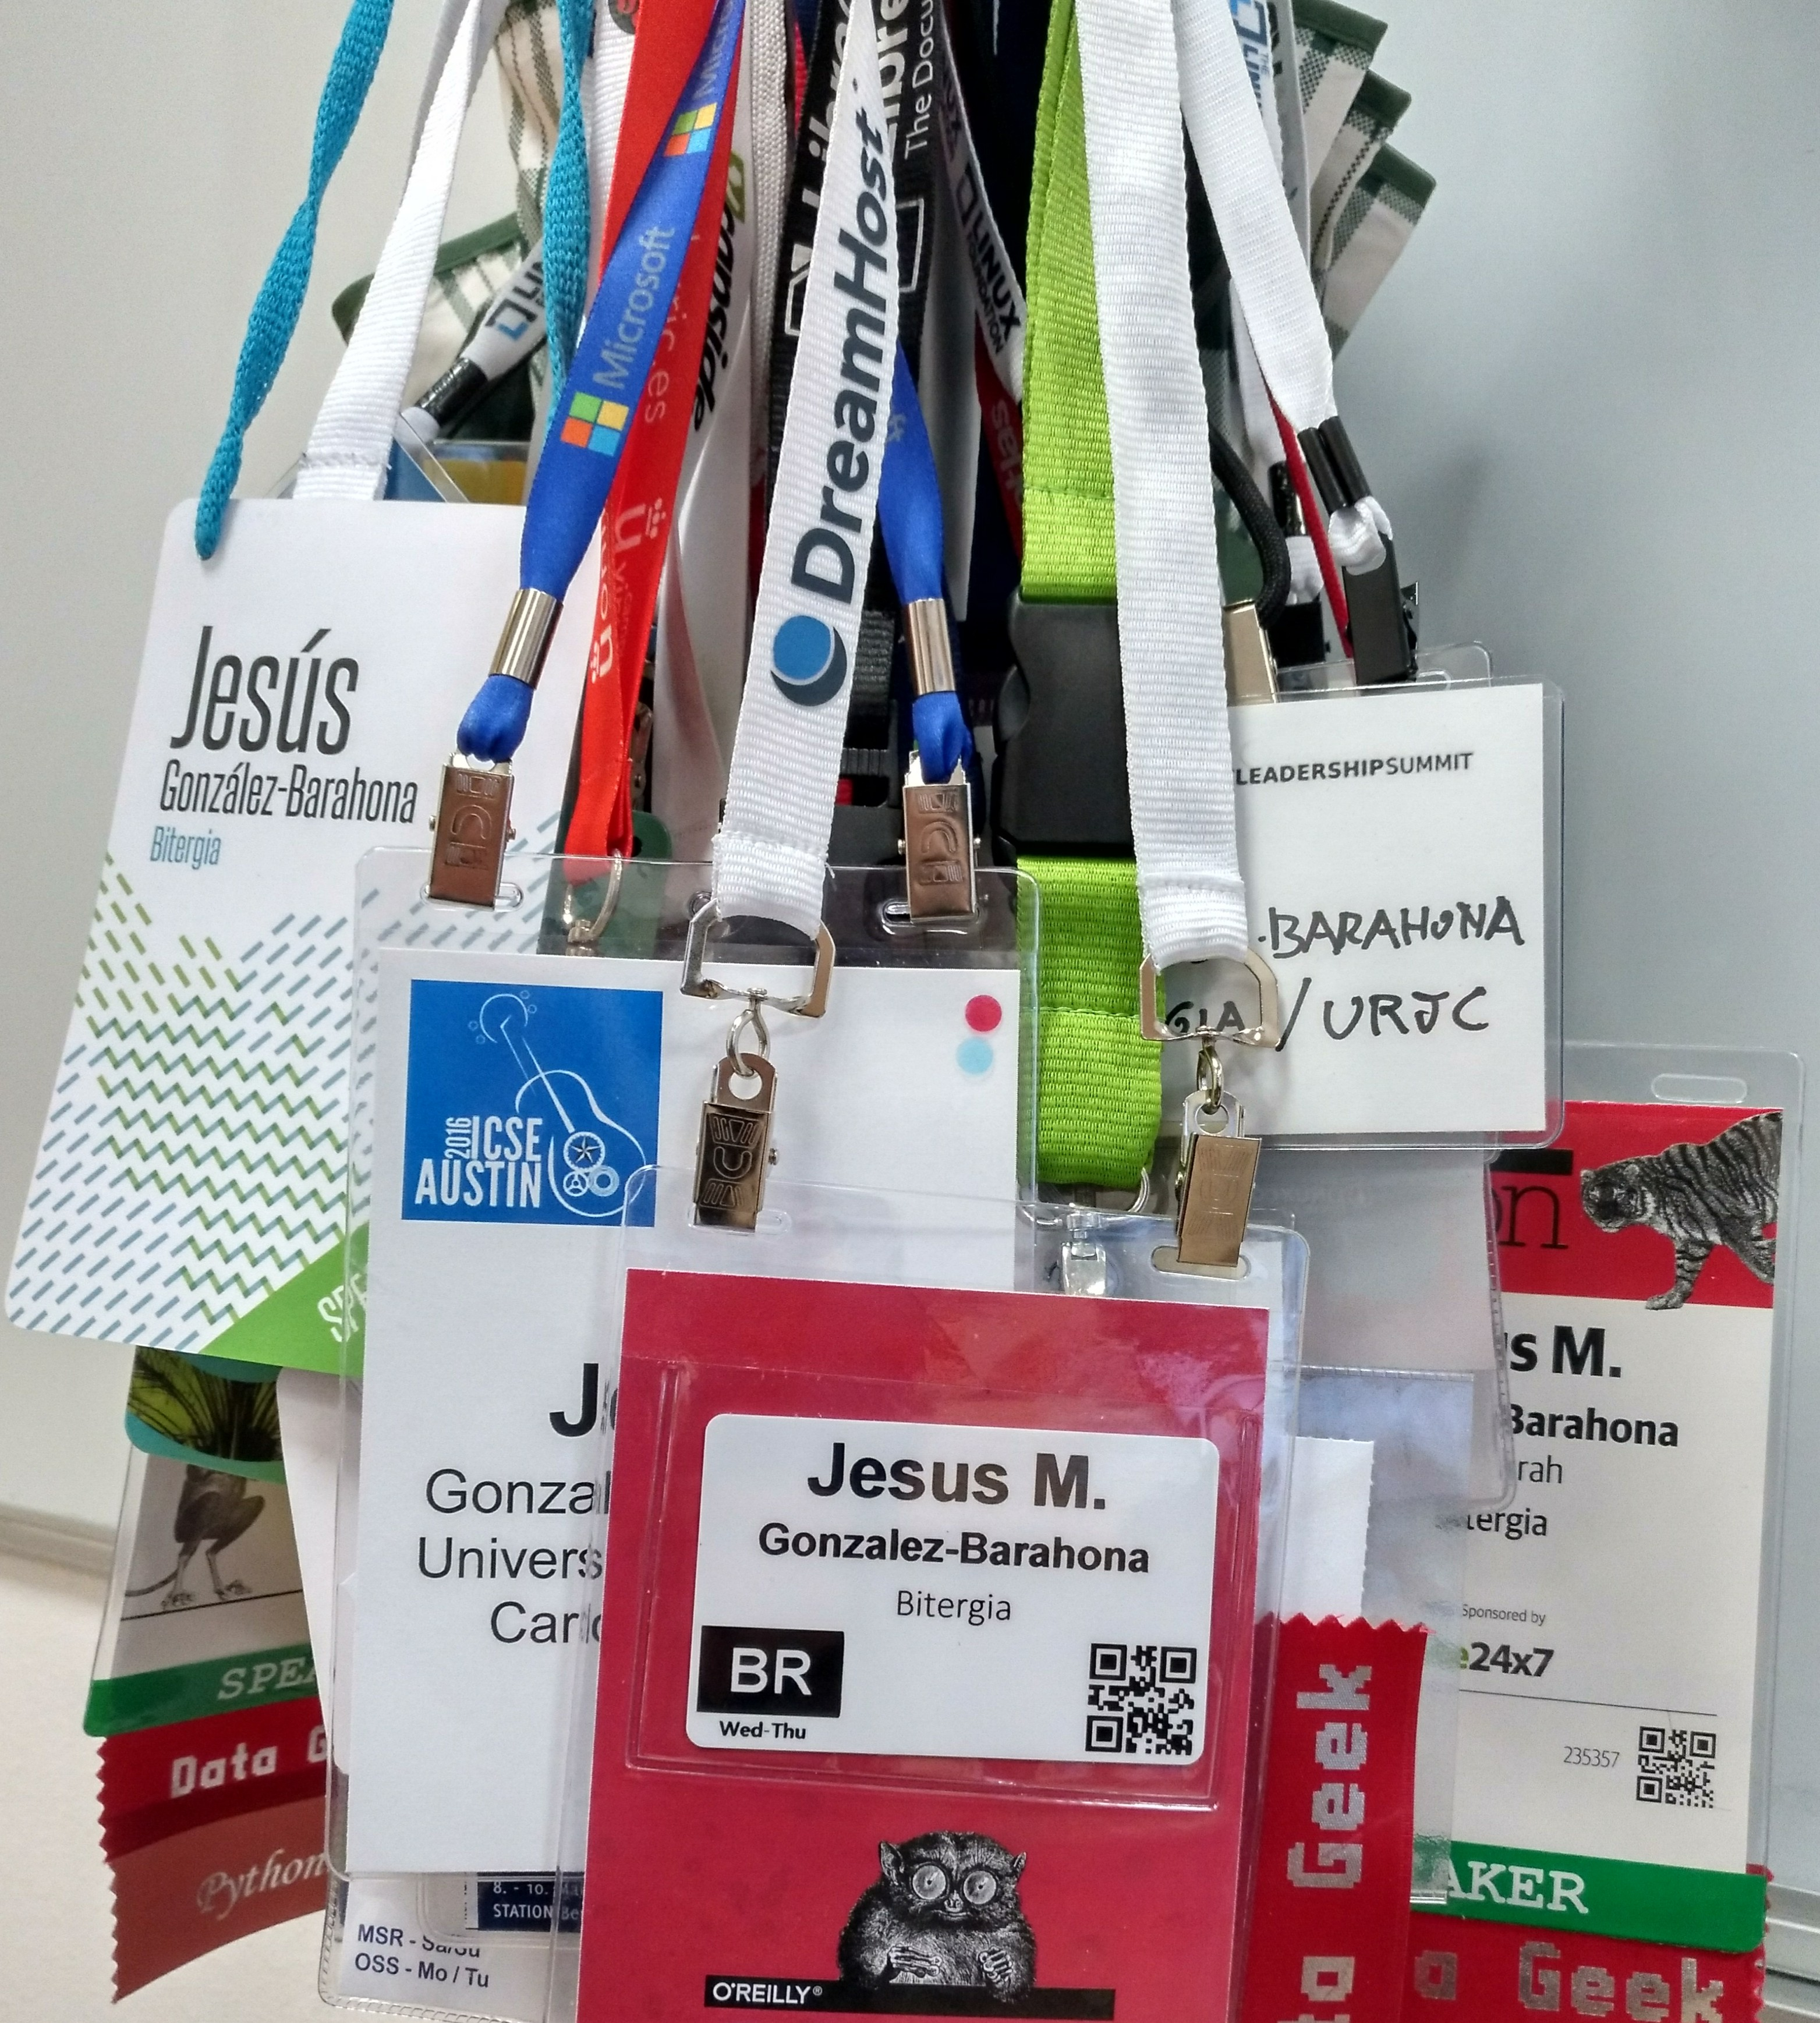
\includegraphics[width=10cm]{figs/badges}
  \end{center}  
  
\end{frame}

%%-----------------------------------------
\begin{frame}[fragile]

  \begin{center}
  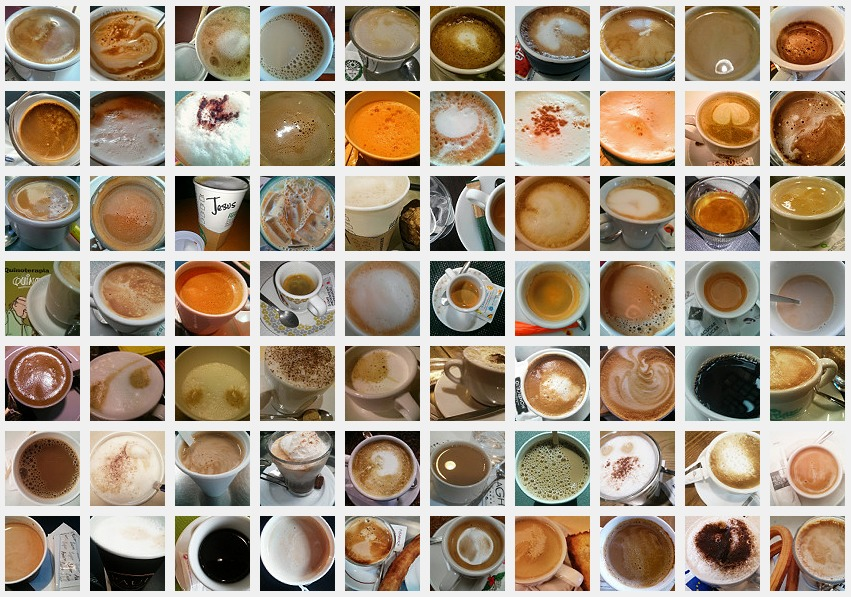
\includegraphics[width=11cm]{figs/coffees}
  \end{center}  
  
\end{frame}

%%-----------------------------------------
\begin{frame}[fragile]

  \begin{center}
    {\em \Large
      Mucha, mucha gente \\
      ha hecho posible \\
      todo esto \\
    }
  \end{center}  
  
\end{frame}

%%-----------------------------------------
\begin{frame}[fragile]

  \begin{center}
    {\em \Huge
      ¡¡Gracias a todos!!
    }
  \end{center}  
  
\end{frame}

%% Presente
%%

\section{Presente}

\begin{flushright}
{\em
  A veces me pregunto \\
  qué hago yo aquí \\
}
~ \\
José Antonio Labordeta \\
\end{flushright}

%%-----------------------------------------
\begin{frame}[fragile]
  \frametitle{Reflexionar}

  \begin{center}
  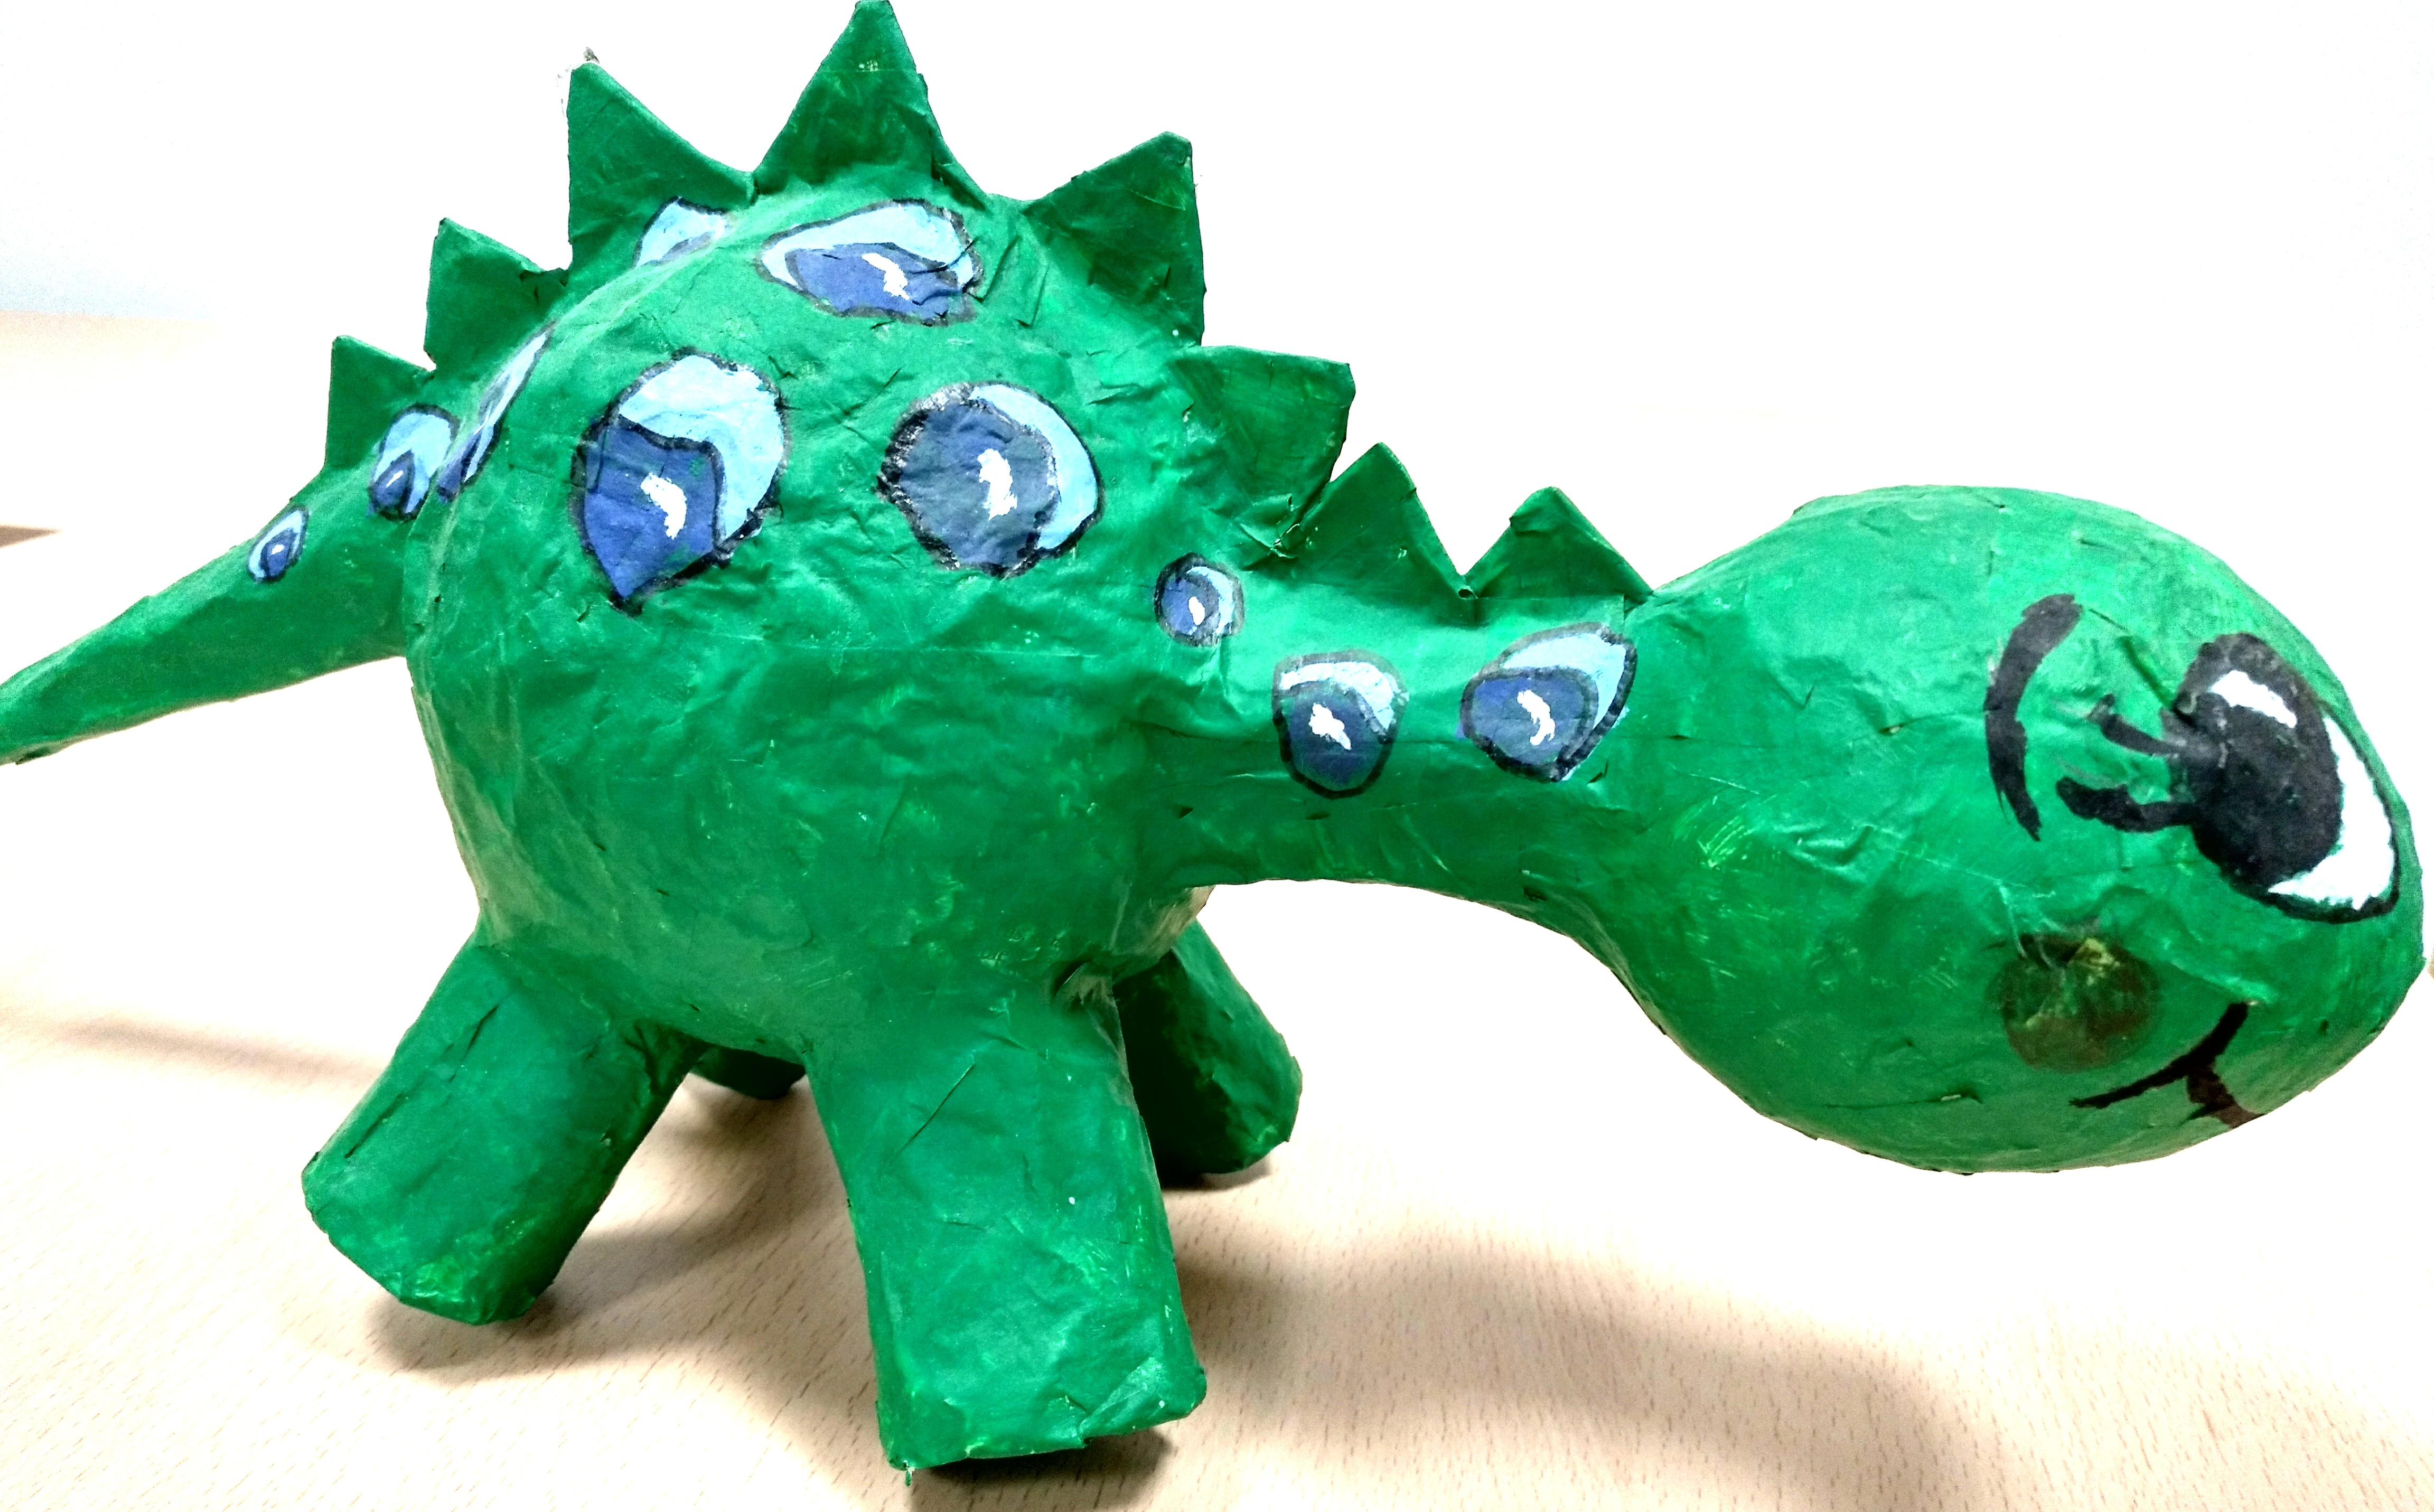
\includegraphics[width=10cm]{figs/dinosaurio}
  \end{center}  
  
\end{frame}

%%-----------------------------------------
\begin{frame}[fragile]
  \frametitle{Aprender}

  \begin{center}
  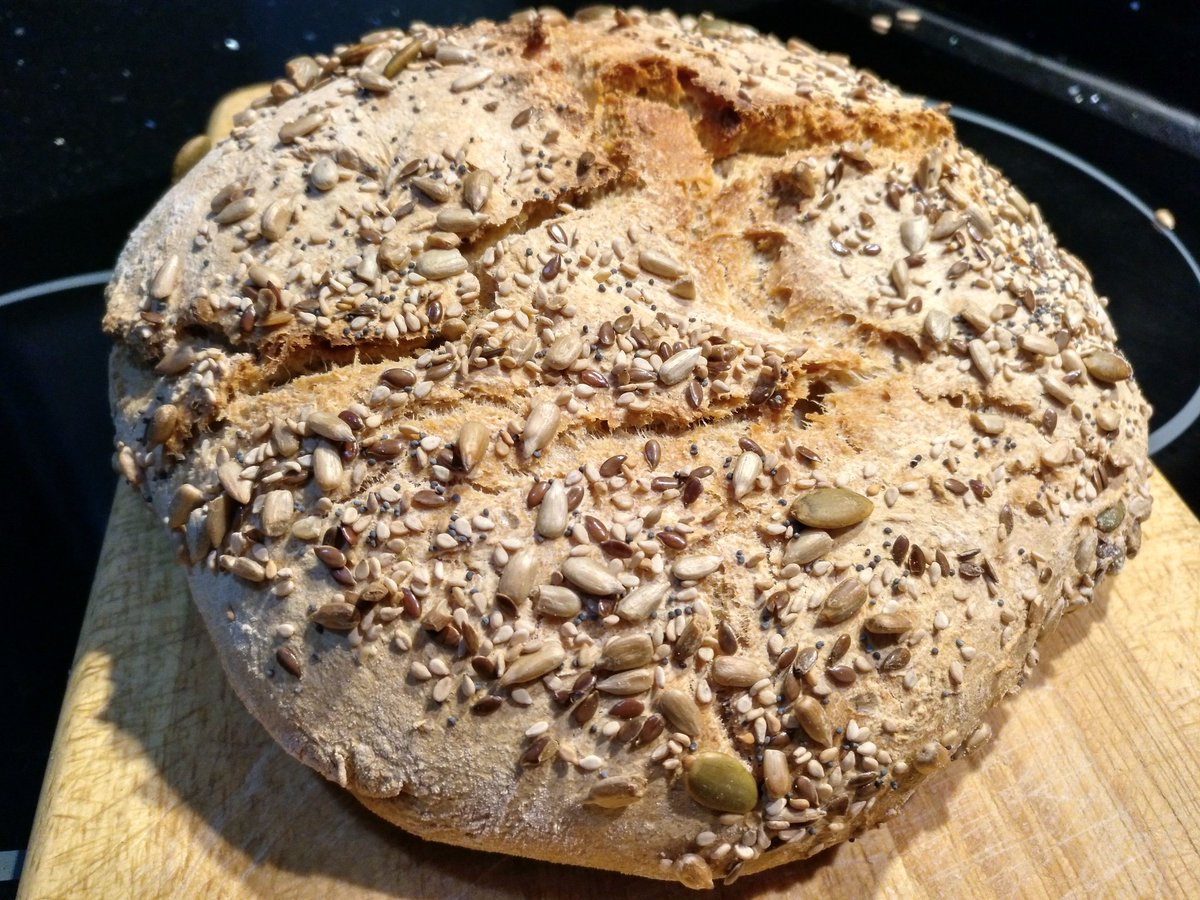
\includegraphics[width=10cm]{figs/pan}
  \end{center}  
  
\end{frame}

%%-----------------------------------------
\begin{frame}[fragile]
  \frametitle{Hacer}

  \begin{center}
  \includegraphics[width=10cm]{figs/anet8}
  \end{center}  
  
\end{frame}

%%-----------------------------------------
\begin{frame}[fragile]
  \frametitle{Explorar}

  \begin{center}
  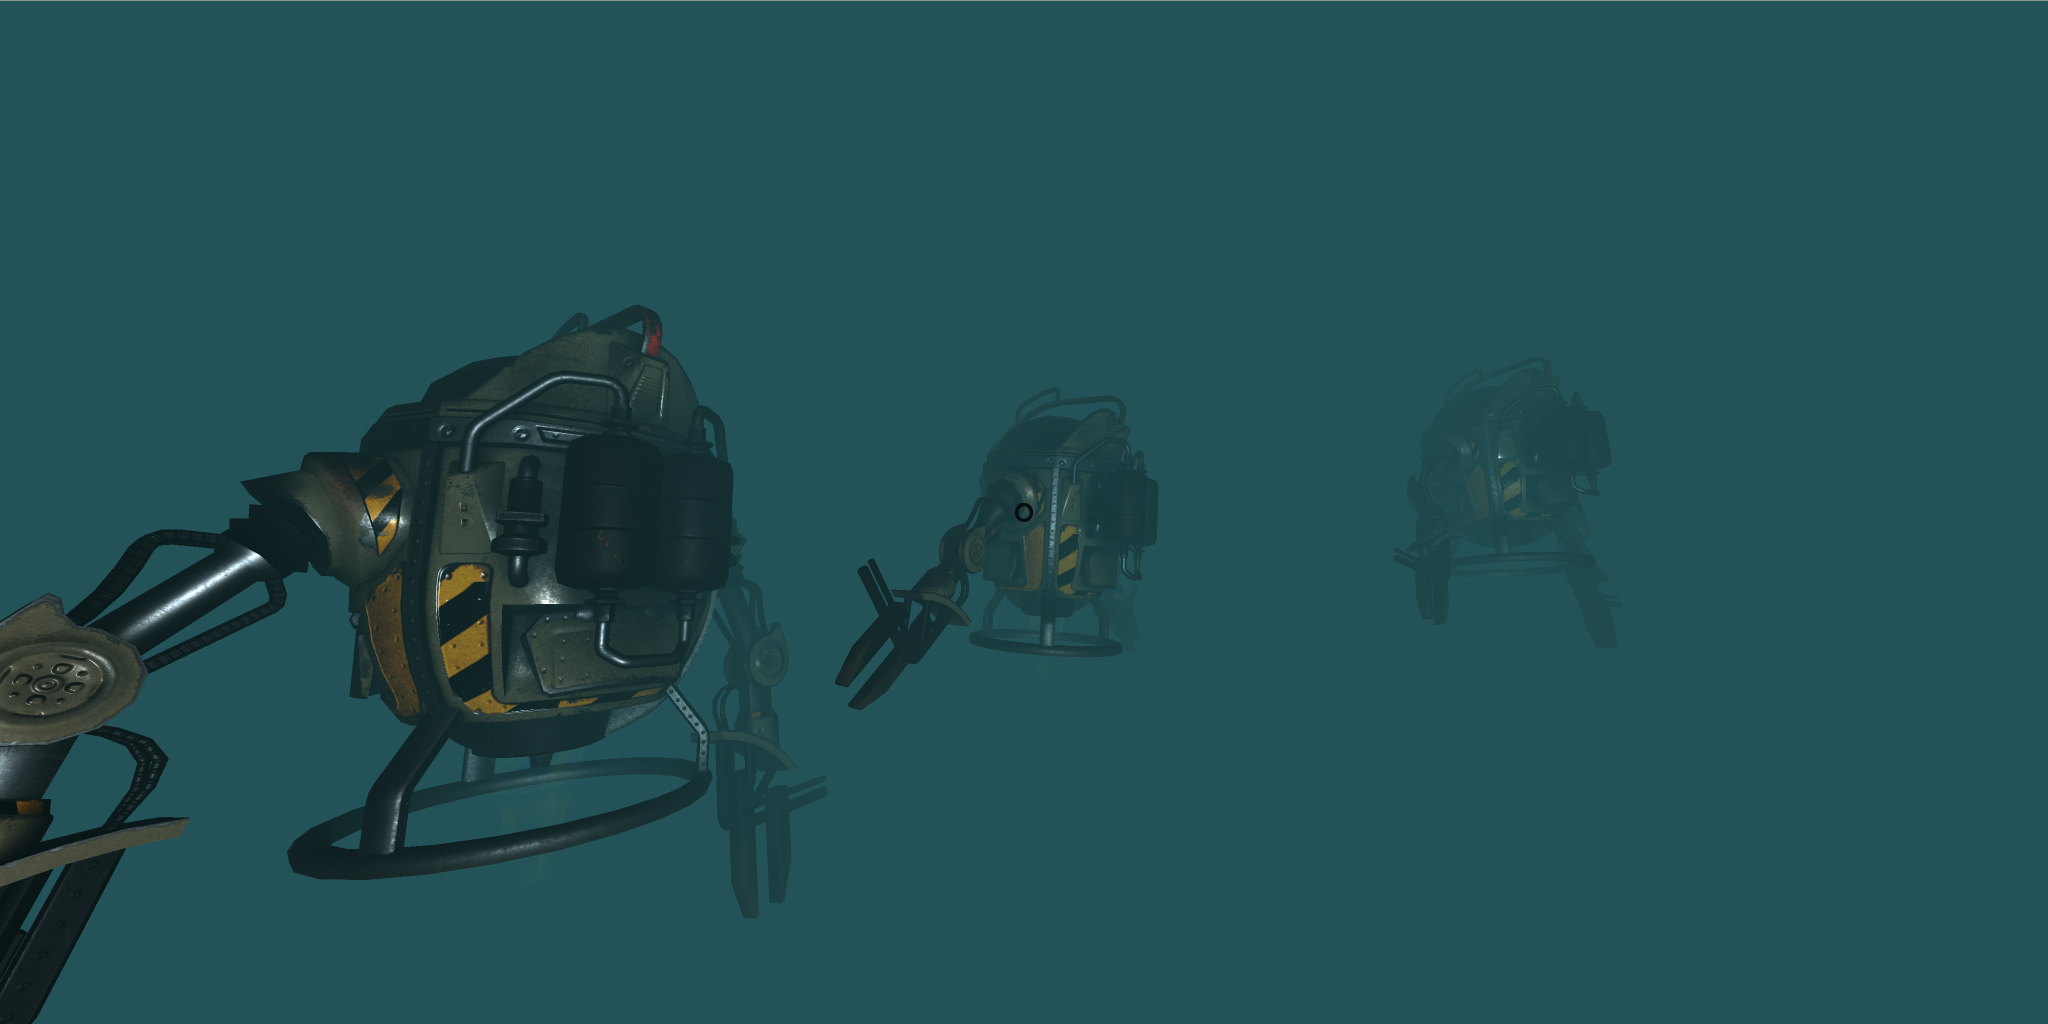
\includegraphics[width=11cm]{figs/aframe-robots}
  \end{center}  
  
\end{frame}

%%-----------------------------------------
\begin{frame}[fragile]
  \frametitle{Contemplar}

  \begin{center}
  \includegraphics[width=10cm]{figs/flor}
  \end{center} 
  
\end{frame}

%% Futuro
%%

\section{Futuro}

\begin{flushright}
{\em
  No hables de futuro \\
  es una ilusión \\
}
~ \\
Loquillo (letra de S. Méndez) \\
\end{flushright}

%%-----------------------------------------
\begin{frame}[fragile]
  \frametitle{Nada está garantizado}

  ``The coming war on general computation'', \\
  Cory Doctorow \\

  \url{https://youtu.be/HUEvRyemKSg}
\end{frame}

%%-----------------------------------------
\begin{frame}[fragile]
  \frametitle{La tecnología no es neutra}


  \url{https://youtu.be/uRXWLLVWVMY}
\end{frame}


%%-----------------------------------------
\begin{frame}[fragile]
  \frametitle{Las cosas están cambiando...}


  ¿Cuál será el próximo modelo de Internet?
  
\end{frame}

%%-----------------------------------------
\begin{frame}[fragile]
  \frametitle{Una apuesta}

  De la nube al suelo

  \begin{center}
  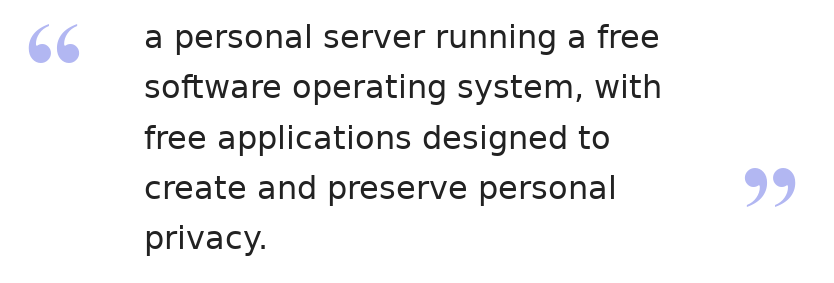
\includegraphics[width=10cm]{figs/freedom-box}
  \end{center}

  Freedom Box
  
\end{frame}
  

%%-----------------------------------------
\begin{frame}[fragile]
  \frametitle{Una apuesta}

  Sistemas VR/AR interconectados

  \begin{center}
  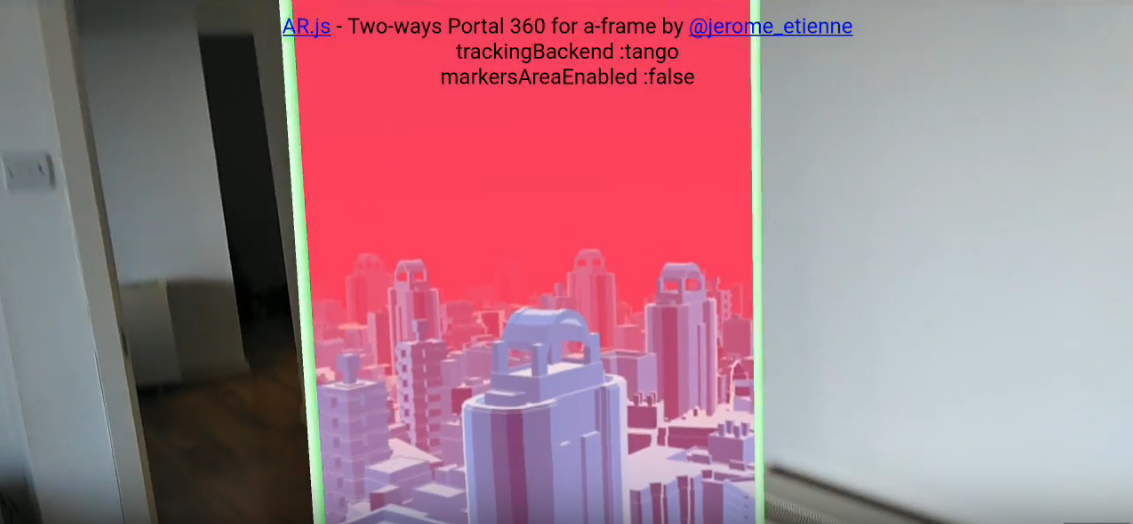
\includegraphics[width=7cm]{figs/aframe-portal}
  \end{center}

  {\small
  \url{https://youtu.be/AI-g2wV9_VA}
  }
  
\end{frame}

%%-----------------------------------------
\begin{frame}[fragile]
  \frametitle{Una apuesta}

  La promesa del peer-to-peer

  \begin{center}
  
\includegraphics[width=7cm]{figs/ipfs}
  
\includegraphics[width=7cm]{figs/webrtc}
  \end{center}
  
\end{frame}

%%-----------------------------------------
\begin{frame}[fragile]
  \frametitle{Una apuesta}

  \begin{center}
  {\Large
  ¿Y si todo esto converge?
  }
  \end{center}
  
\end{frame}


\frame{
~
\vspace{1cm}

\begin{flushright}


\includegraphics[width=2.2cm]{figs/by-sa}
 \\

\begin{footnotesize}
\copyright 2018 Jesús M. González Barahona. \\

\vspace{.4cm}

Algunos derechos reservados. Este artículo se distribuye bajo
la licencia ``Reconocimiento-CompartirIgual 4.0 España'' de Creative Commons,
disponible en \\
{\scriptsize \url{http://creativecommons.org/licenses/by-sa/4.0/es/deed.es}} \\

\vspace{.4cm}

Este documento (o uno muy similar) está disponible en \\
\url{http://github.com/jgbarah/presentaciones}

\end{footnotesize}
\end{flushright}

}
%%

%\againframe{firstframe}

\end{document}
